%\RequirePackage[l2tabu, orthodox]{nag}
\RequirePackage{currfile}
\documentclass[12pt]{beamer}
\graphicspath{{Imagenes/}{../Imagenes/}}
\usepackage[utf8]{inputenc}
\usepackage[spanish]{babel}
\usepackage{standalone}
\usepackage{color}
\usepackage[binary-units=true]{siunitx}
\usepackage{hyperref}
\hypersetup{
  colorlinks=true,
  linkcolor=blue,          % color of internal links (change box color with linkbordercolor)
  citecolor=green,        % color of links to bibliography
  filecolor=magenta,      % color of file links
  urlcolor=cyan,           % color of external links
  linkbordercolor={0 0 1}
}
\usepackage{xcolor, soul}
\usepackage{etoolbox}
\usepackage{amsmath}
\usepackage{amsthm}
\usepackage{physics}
\usepackage{multicol}
\usepackage{graphicx}
\usepackage{bookmark}
\usepackage{longtable}
\usepackage{graphicx}
\usepackage{tikz}
\usepackage[siunitx, RPvoltages]{circuitikz}
\usetikzlibrary{mindmap}
\usetikzlibrary{arrows, patterns, shapes, decorations.markings, decorations.pathmorphing}
\usetikzlibrary{matrix,positioning}
\tikzstyle{every picture}+=[remember picture,baseline]
\usepackage[autostyle,spanish=mexican]{csquotes}
\usepackage{pifont}
\usepackage[font=footnotesize,textfont=it]{caption}
\usepackage{tabulary}
\usepackage{booktabs}
\usepackage[outdir=./]{epstopdf}
%\usepackage{epstopdf}
\usepackage{media9}
\usepackage{multimedia}
\usepackage{bigints}
%\usepackage{enumitem}
\usepackage[os=win]{menukeys}
\usepackage{pifont}
\usepackage{pbox}
\usepackage{alltt}
\usepackage{verbatim}
\usepackage{colortbl}
\usepackage{tcolorbox}
\usepackage{fancyvrb}
\usepackage[sfdefault]{roboto}  %% Option 'sfdefault' only if the base font of the document is to be sans serif
%\usepackage[T1]{fontenc}
\setcounter{secnumdepth}{3}
\setcounter{tocdepth}{3}
\DeclareGraphicsExtensions{.pdf,.png,.jpg}
\renewcommand {\arraystretch}{1.5}
\definecolor{ao}{rgb}{0.0, 0.5, 0.0}
\definecolor{aquamarine}{rgb}{0.5, 1.0, 0.83}
\definecolor{kellygreen}{rgb}{0.3, 0.73, 0.09}
\definecolor{bisque}{rgb}{1.0, 0.89, 0.77}
\definecolor{amber}{rgb}{1.0, 0.75, 0.0}
\definecolor{armygreen}{rgb}{0.29, 0.33, 0.13}
\definecolor{alizarin}{rgb}{0.82, 0.1, 0.26}
\definecolor{cadetblue}{rgb}{0.37, 0.62, 0.63}
\newcommand*{\TitleParbox}[1]{\parbox[c]{6cm}{\raggedright #1}}%
\newcommand{\python}{\texttt{python}}
\newcommand{\textoazul}[1]{\textcolor{blue}{#1}}
\newcommand{\azulfuerte}[1]{\textcolor{blue}{\textbf{#1}}}
\newcommand{\funcionazul}[1]{\textcolor{blue}{\textbf{\texttt{#1}}}}
%\normalfont
\usepackage{ccfonts}% http://ctan.org/pkg/{ccfonts}
\usepackage[T1]{fontenc}% http://ctan.or/pkg/fontenc
\renewcommand{\rmdefault}{cmr}% cmr = Computer Modern Roman
\usefonttheme[onlymath]{serif}
\linespread{1.3}
\newcounter{saveenumi}
\newcommand{\seti}{\setcounter{saveenumi}{\value{enumi}}}
\newcommand{\conti}{\setcounter{enumi}{\value{saveenumi}}}
\newcommand{\tikzmark}[1]{\tikz[remember picture] \node[coordinate] (#1) {#1};}

\usepackage{scalerel}[2016-12-29]
\def\stretchint#1{\vcenter{\hbox{\stretchto[440]{\displaystyle\int}{#1}}}}
\def\scaleint#1{\vcenter{\hbox{\scaleto[3ex]{\displaystyle\int}{#1}}}}
\def\bs{\mkern-12mu}

\newtheorem{teo}{}[section]
\usepackage{blkarray}

%reduce el tamaño de letra de la etiqueta equations
\makeatletter
\def\maketag@@@#1{\hbox{\m@th\normalfont\small#1}}
\makeatother

%se usa para la x en itemize
\newcommand{\xmark}{\text{\ding{55}}}

%\AtBeginDocument{\setlength{\tymin}{1em}}


\definecolor{myblue}{rgb}{.8, .8, 1}

\usepackage{empheq}

\newlength\mytemplen
\newsavebox\mytempbox

\makeatletter
\newcommand\mybluebox{%
    \@ifnextchar[%]
       {\@mybluebox}%
       {\@mybluebox[0pt]}}

\def\@mybluebox[#1]{%
    \@ifnextchar[%]
       {\@@mybluebox[#1]}%
       {\@@mybluebox[#1][0pt]}}

\def\@@mybluebox[#1][#2]#3{
    \sbox\mytempbox{#3}%
    \mytemplen\ht\mytempbox
    \advance\mytemplen #1\relax
    \ht\mytempbox\mytemplen
    \mytemplen\dp\mytempbox
    \advance\mytemplen #2\relax
    \dp\mytempbox\mytemplen
    \colorbox{myblue}{\hspace{1em}\usebox{\mytempbox}\hspace{1em}}}

\makeatother



%Se usa la plantilla Warsaw modificada con whale
\mode<presentation>
{
  \usetheme{Warsaw}
  \setbeamertemplate{headline}{}
  %\useoutertheme{infolines}
  \usecolortheme{whale}
  \setbeamercovered{invisible}
  

 \setbeamertemplate{section in toc}[sections numbered]
 \setbeamertemplate{subsection in toc}[subsections numbered]
 \setbeamertemplate{subsection in toc}{\leavevmode\leftskip=3.2em\rlap{\hskip-2em\inserttocsectionnumber.\inserttocsubsectionnumber}\inserttocsubsection\par}
% \setbeamercolor{section in toc}{fg=blue}
 \setbeamercolor{subsection in toc}{fg=blue}
 \setbeamerfont{subsection in toc}{size=\small}


\setbeamertemplate{navigation symbols}{}
\setbeamertemplate{caption}[numbered]
% \setbeamercolor{frametitle}{fg=yellow,bg=blue!70!white}
\setbeamercolor{section in head/foot}{bg=black, fg=white}
%\setbeamercolor{subsection in head/foot}{bg=gray!30,fg=black}
%\setbeamercolor{author in head/foot}{fg=yellow}
%\setbeamercolor{date in head/foot}{fg=blue}

%\mode<presentation>
%{
%  \usetheme{Warsaw}
%  \setbeamertemplate{headline}{}
%  %\useoutertheme{infolines}
%  \useoutertheme{default}
%  \setbeamercovered{invisible}
%  % or whatever (possibly just delete it)
%}
}


\usepackage{courier}
\usepackage{listingsutf8}
\usepackage{listings}
\usepackage{xcolor}
\usepackage{textcomp}
\usepackage{color}
\definecolor{deepblue}{rgb}{0,0,0.5}
\definecolor{brown}{rgb}{0.59, 0.29, 0.0}
\definecolor{OliveGreen}{rgb}{0,0.25,0}
% \usepackage{minted}

\DeclareCaptionFont{white}{\color{white}}
\DeclareCaptionFormat{listing}{\colorbox{gray}{\parbox{0.98\textwidth}{#1#2#3}}}
\captionsetup[lstlisting]{format=listing,labelfont=white,textfont=white}
\renewcommand{\lstlistingname}{Código}


\definecolor{Code}{rgb}{0,0,0}
\definecolor{Keywords}{rgb}{255,0,0}
\definecolor{Strings}{rgb}{255,0,255}
\definecolor{Comments}{rgb}{0,0,255}
\definecolor{Numbers}{rgb}{255,128,0}

\makeatletter

\newif\iffirstchar\firstchartrue
\newif\ifstartedbyadigit
\newif\ifprecededbyequalsign

\newcommand\processletter
{%
  \ifnum\lst@mode=\lst@Pmode%
    \iffirstchar%
        \global\startedbyadigitfalse%
      \fi
      \global\firstcharfalse%
    \fi
}

\newcommand\processdigit
{%
  \ifnum\lst@mode=\lst@Pmode%
      \iffirstchar%
        \global\startedbyadigittrue%
      \fi
      \global\firstcharfalse%
  \fi
}

\lst@AddToHook{OutputOther}%
{%
  \lst@IfLastOtherOneOf{=}
    {\global\precededbyequalsigntrue}
    {}%
}

\lst@AddToHook{Output}%
{%
  \ifprecededbyequalsign%
      \ifstartedbyadigit%
        \def\lst@thestyle{\color{orange}}%
      \fi
    \fi
  \global\firstchartrue%
  \global\startedbyadigitfalse%
  \global\precededbyequalsignfalse%
}

\lstset{ 
language=Python,                % choose the language of the code
basicstyle=\footnotesize\ttfamily,       % the size of the fonts that are used for the code
numbers=left,                   % where to put the line-numbers
numberstyle=\scriptsize,      % the size of the fonts that are used for the line-numbers
stepnumber=1,                   % the step between two line-numbers. If it is 1 each line will be numbered
numbersep=5pt,                  % how far the line-numbers are from the code
backgroundcolor=\color{white},  % choose the background color. You must add \usepackage{color}
showspaces=false,               % show spaces adding particular underscores
showstringspaces=false,         % underline spaces within strings
showtabs=false,                 % show tabs within strings adding particular underscores
frame=single,   		% adds a frame around the code
tabsize=2,  		% sets default tabsize to 2 spaces
captionpos=t,   		% sets the caption-position to bottom
breaklines=true,    	% sets automatic line breaking
breakatwhitespace=false,    % sets if automatic breaks should only happen at whitespace
escapeinside={\#},  % if you want to add a comment within your code
stringstyle =\color{OliveGreen},
%otherkeywords={{as}},             % Add keywords here
keywordstyle = \color{blue},
commentstyle = \color{black},
identifierstyle = \color{black},
literate=%
         {á}{{\'a}}1
         {é}{{\'e}}1
         {í}{{\'i}}1
         {ó}{{\'o}}1
         {ú}{{\'u}}1
%
%keywordstyle=\ttb\color{deepblue}
%fancyvrb = true,
}

\lstdefinestyle{FormattedNumber}{%
    literate={0}{{\textcolor{red}{0}}}{1}%
             {1}{{\textcolor{red}{1}}}{1}%
             {2}{{\textcolor{red}{2}}}{1}%
             {3}{{\textcolor{red}{3}}}{1}%
             {4}{{\textcolor{red}{4}}}{1}%
             {5}{{\textcolor{red}{5}}}{1}%
             {6}{{\textcolor{red}{6}}}{1}%
             {7}{{\textcolor{red}{7}}}{1}%
             {8}{{\textcolor{red}{8}}}{1}%
             {9}{{\textcolor{red}{9}}}{1}%
             {.0}{{\textcolor{red}{.0}}}{2}% Following is to ensure that only periods
             {.1}{{\textcolor{red}{.1}}}{2}% followed by a digit are changed.
             {.2}{{\textcolor{red}{.2}}}{2}%
             {.3}{{\textcolor{red}{.3}}}{2}%
             {.4}{{\textcolor{red}{.4}}}{2}%
             {.5}{{\textcolor{red}{.5}}}{2}%
             {.6}{{\textcolor{red}{.6}}}{2}%
             {.7}{{\textcolor{red}{.7}}}{2}%
             {.8}{{\textcolor{red}{.8}}}{2}%
             {.9}{{\textcolor{red}{.9}}}{2}%
             {\ }{{ }}{1}% handle the space
         ,%
          %mathescape=true
          escapeinside={__}
          }



\makeatletter

% \setbeamercolor{subsection in foot}{bg=blue!30!yellow, fg=red}
%\setbeamercolor{footlinecolor}{bg=black,fg=white}
\setbeamertemplate{footline}
{
  \leavevmode%
  \hbox{%
  \begin{beamercolorbox}[wd=.333333\paperwidth,ht=2.25ex,dp=1ex,center]{section in footline}%
    \usebeamerfont{section in foot} \insertsection
  \end{beamercolorbox}}%
  \begin{beamercolorbox}[wd=.333333\paperwidth,ht=2.25ex,dp=1ex,center]{subsection in foot}%
    \usebeamerfont{subsection in foot}  \insertsubsection
  \end{beamercolorbox}%
  \begin{beamercolorbox}[wd=.333333\paperwidth,ht=2.25ex,dp=1ex,right]{date in head/foot}%
    \usebeamerfont{date in head/foot} \insertshortdate{} \hspace*{2em}
    \insertframenumber{} / \inserttotalframenumber \hspace*{2ex} 
  \end{beamercolorbox}}%
  \vskip0pt%
\makeatother
\normalfont
\usepackage{ccfonts}% http://ctan.org/pkg/{ccfonts}
\usepackage[T1]{fontenc}% http://ctan.or/pkg/fontenc
\renewcommand{\rmdefault}{cmr}% cmr = Computer Modern Roman
\linespread{1.3}
\title{EDO con condiciones de frontera}
\subtitle{Curso de Física Computacional}
\author{M. en C. Gustavo Contreras Mayén}
\date{\today}
\institute{Facultad de Ciencias - UNAM}
\titlegraphic{
\includegraphics[width=1.75cm]{Imagenes/escudo-facultad-ciencias.jpg}\hspace*{4.75cm}~%
   
\includegraphics[width=1.75cm]{Imagenes/escudo-unam.jpg}
}
\begin{document}
\maketitle
\fontsize{14}{14}\selectfont
\spanishdecimal{.}
\section*{Contenido}
\frame{\tableofcontents[currentsection, hideallsubsections]}
\section{EDO con condiciones de frontera}
\frame{\tableofcontents[currentsection, hideothersubsections]}
\subsection{Consideraciones}
\begin{frame}
\frametitle{ED con condiciones en la frontera}
En problemas con ED con valores en dos puntos, las condiciones auxiliares asociadas con la ecuación diferencial, denominadas \emph{condiciones de frontera}, se especifican en dos valores diferentes de $x$.
\[  y^{\prime \prime} = f(x, y, y^{\prime}), \hspace{1cm} y(a) = \alpha, \hspace{1cm} y(b) = \beta \]
\end{frame}
\begin{frame}
\frametitle{ED con condiciones en la frontera}
Esta aparentemente pequeña modificación de los problemas de valor inicial tiene una repercusión mayor: hace que los problemas de los valores en la frontera sean considerablemente más difíciles de resolver.
\end{frame}
\begin{frame}
\frametitle{ED con condiciones en la frontera}
En un problema de ED con valor inicial comenzamos en el punto donde se dieron los valores iniciales y avanzar la solución hacia adelante en la medida en que sea necesario.
\\
\bigskip
Esta técnica no funciona para problemas de valores en la frontera, ya que no hay suficientes condiciones iniciales disponibles en ninguno de los extremos para producir una solución única.
\end{frame}
\begin{frame}
\frametitle{ED con condiciones en la frontera}
Una manera de superar la falta de condiciones iniciales es \enquote{adivinar/suponer} los valores perdidos.
\\
\bigskip
Es muy poco probable que la solución resultante satisfaga las condiciones de frontera en el otro extremo, pero al inspeccionar la diferencia podemos estimar qué cambios habrá que reazliar en las condiciones iniciales antes de integrar nuevamente.
\end{frame}
\begin{frame}
\frametitle{El método de disparo}
Este procedimiento iterativo se conoce como el \textcolor{blue}{método de disparo}. 
\\
\bigskip
El nombre se deriva de la analogía con el tiro al blanco: haz un tiro y observa donde golpea al objetivo; luego corrije el objetivo y vuelva a disparar.
\end{frame}
\begin{frame}
\frametitle{Método de diferencias finitas}
Otro método para resolver problemas de ED con valores en la frontera es el \textcolor{blue}{método de diferencias finitas}, donde las ED son aproximadas por diferencias finitas en puntos de una malla uniformemente espaciados.
\\
\bigskip
Como consecuencia, una ED se transforma en un conjunto de ecuaciones algebraicas simultáneas.
\end{frame}
\begin{frame}
\frametitle{Sistemas no lineales}
Los dos métodos mencionados tienen un problema común: \textcolor{red}{generan un conjunto de ecuaciones no lineales, si las ecuaciones diferenciales son no lineales}.
\end{frame}
\begin{frame}
\frametitle{Solución de sistemas no lineales}
Los métodos para resolver ecuaciones no lineales son procedimientos iterativos que pueden consumir una gran cantidad de recursos computacionales.
\\
\bigskip
Por lo que resolver problemas de ED no lineales CDF no es barato. Otra complicación es que los métodos iterativos necesitan valores de partida razonablemente buenos para converger. 
\end{frame}
\section{Método de disparo}
\frame{\tableofcontents[currentsection, hideothersubsections]}
\subsection{Definición del método de disparo}
\begin{frame}
\frametitle{Método de disparo}
El problema más simple de condiciones en la frontera es una \textoazul{EDO2} con una condición especificada en $x = a$ y otra en $x = b$.
\begin{equation}
y^{\prime \prime} = f(x, y, y^{\prime}) \hspace{1cm} y(a) = \alpha, \hspace{0.5cm} y(b) = \beta
\label{eq:ecuacion_08_01}
\end{equation}
\end{frame}
\begin{frame}
\frametitle{Propuesta de solución}
Hagamos el intento de cambiar la ecuación (\ref{eq:ecuacion_08_01}) en un problema de valores iniciales
\begin{equation}
y^{\prime \prime} = f(x, y, y^{\prime}) \hspace{1cm} y(a) = \alpha, \hspace{0.5cm} y^{\prime}(a) = u
\label{eq:ecuacion_08_02}
\end{equation}
\end{frame}
\begin{frame}
\frametitle{Propuesta de solución}
El punto importante es encontrar el valor correcto de $u$.
\\
\bigskip
Esto podría hacerse por ensayo y error: Supongo $u$ y resuelvo el problema de valor inicial avanzando desde $x = a$ hasta $b$.
\end{frame}
\begin{frame}
\frametitle{Propuesta de solución}
\begin{itemize}[<+->]
\item Si la solución coincide con la condición de frontera prescrita $y(b) = \beta$, ya la hicimos!!
\item De lo contrario tenemos que ajustar el valor de $u$ y volver a intentarlo.
\end{itemize}
\pause
Claramente, este procedimiento es muy tedioso.
\end{frame}
\begin{frame}
\frametitle{Simplificación del problema}
Podemos ser más sistemáticos si nos damos cuenta de que para encontrar el valor correcto de $u$, \emph{es un problema de búsqueda de raíces}.
\end{frame}
\begin{frame}
\frametitle{Simplificación del problema}
Como la solución del problema de valor inicial depende de $u$, el valor calculado de $y(b)$ es una función de $u$; es decir
\[ y(b) = \theta(u) \]
\end{frame}
\begin{frame}
\frametitle{Simplificación del problema}
\[ y(b) = \theta(u) \]
donde $u$ es una raíz de
\begin{equation}
r(u) = \theta(u) - \beta = 0
\label{eq:ecuacion_08_03}
\end{equation}
donde $r(u)$ es el residual de frontera: es la diferencia entre el valor de frontera calculado y el que se especifica en $x=b$.
\end{frame}
\begin{frame}
\frametitle{Simplificación del problema}
Podemos resolver la ecuación (\ref{eq:ecuacion_08_03}) a partir de cualquiera de los métodos discutidos en el Tema 2 de Operaciones Matemáticas Básicas, pero toma en cuenta que:
\pause
\begin{itemize}[<+->]
\item El método de bisección no debe de utilizarse ya que involucra demasiadas evaluaciones de $\theta(u)$.
\item El método de Newton-Rapshon requiere que conozcamos $d \theta / d u$, lo que no podría hacerse de manera sencilla.
\end{itemize}
\end{frame}
\begin{frame}
\frametitle{Calculando raíces}
Toma en cuenta que si la ED es lineal, cualquier método para calcular la raíz necesitará solamente una interpolación para determinar el valor de $u$.
\end{frame}
\subsection{Ejemplo}
\begin{frame}
\frametitle{Ejemplo}
Hagamos un ejercicio para revisar el método. Sea la siguiente EDO-2
\begin{equation}
u^{\prime \prime} = - \dfrac{\pi^{2}}{4}(u + 1)
\end{equation}
y las CDF son $u(0) = 0$ y $u(1) = 1$. 
\\
\bigskip
\pause
Definimos $y_{1} = u$ y $y_{2} = u^{\prime}$, por lo que tenemos ahora
\begin{align*}
\dfrac{dy_{1}}{dx} &= y_{2} \\
\dfrac{dy_{2}}{dx} &= - \dfrac{\pi^{2}}{4}(y_{1} + 1)
\end{align*}
\end{frame}
\begin{frame}
Asumimos que la ecuación tiene los valores iniciales $y_{1}(0) = 0$ y $y_{2}(0) = \alpha$.
\\
\bigskip
\pause
El valor de $\alpha$ tendrá que ajustarse para que $f(\alpha) = u_{\alpha}(1) - 1 = 0$.
\\
\bigskip
Podemos combinar el método de la secante y resolver el sistema de \textcolor{blue}{1-EDO} como lo hemos venido haciendo.
\end{frame}
\begin{frame}
\frametitle{Solución analítica de la EDO-CDF}
El problema CDF se resuelve de manera exacta, la solución analítica es:
\begin{equation}
u(x) = \cos\left(\frac{x \pi}{2}\right) + 2 \sin \left(\frac{x \pi}{2}\right) -1
\end{equation}
\end{frame}
\begin{frame}[plain, allowframebreaks, fragile]
\frametitle{Código para la solución}
\begin{lstlisting}[caption=Código para el método de disparo, style=FormattedNumber, basicstyle=\linespread{1.1}\ttfamily=\small, columns=fullflexible]
def F(y,x):
    F = np.zeros((2), dtype='float_64_')
    F[_0_] = y[_1_]
    F[_1_] = - (np.pi * np.pi)/4.*(y[_0_] + 1.)
    return F

def exacta(x):
    return np.cos(np.pi * (x/2.)) + 2 * np.sin(np.pi * (x/2.)) - 1


y_0_ = np.array([0.0, 1.0])

x = np.linspace(0.0, 1.0)

y_1_ = odeint(F, y_0_, x)

for i in range(len(y_1_)):
    print ('{:1.6f} \t {:1.6f}'.format(x[i], y_1_[:,_0_][i]))

plt.plot(x,y_1_[:,_0_],'r+', label='solucion con alfa de prueba')
plt.plot(x,exacta(x),'b-', label='solucion exacta')
plt.xlabel('x')
plt.ylabel('u(x)')
plt.title('Metodo de disparo con $\alpha = 1.0$')
plt.xlim(0, 1)
plt.axhline(y = 0, color='k', lw=0.75, ls='dashed')
plt.legend(loc='lower left', bbox_\textunderscore_to_\textunderscore_anchor=(0.5, 0.35))
plt.show()
\end{lstlisting}
\end{frame}
\begin{frame}[fragile]
\frametitle{Solución con $y0 = array([0.0,\alpha=1.0])$}
\begin{figure}
    \centering
    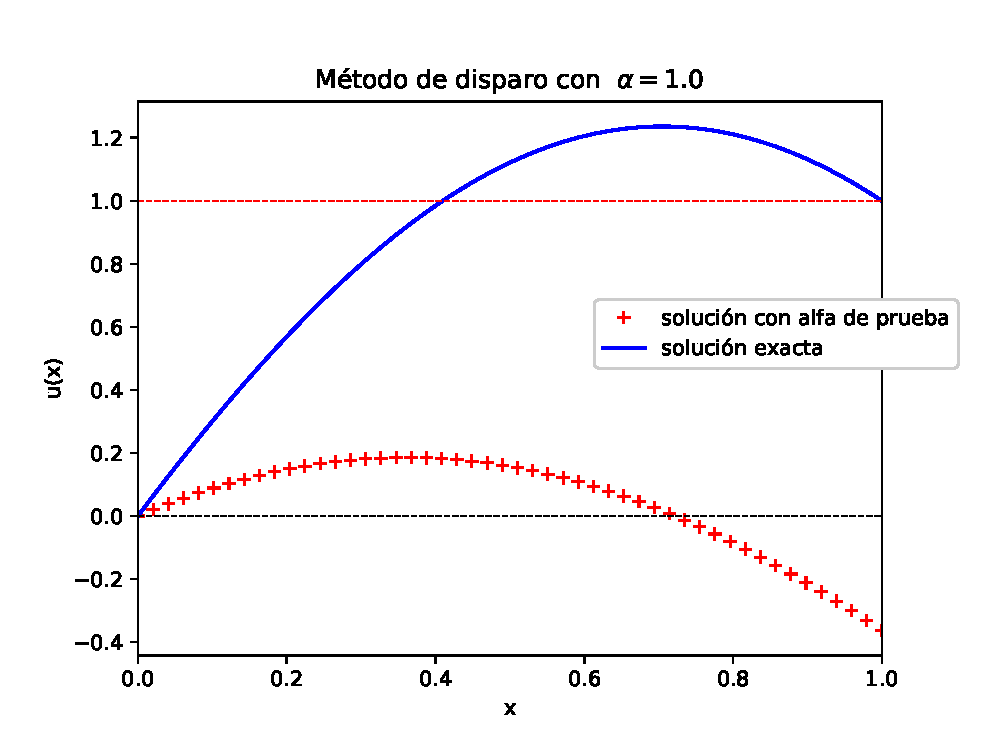
\includegraphics[scale=0.6]{MetodoDisparo2017_01.eps}
\end{figure}
\end{frame}
\begin{frame}
\frametitle{Cambio en el parámetro}
Como el valor de $\alpha = 1$ nos devuelve una solución que comparada con la solución exacta, queda muy por debajo del valor de la condición de frontera del lado derecho.
\\
\bigskip
Por lo que hay que modificar el valor, probamos ahora con un valor de $\alpha = 4.0$, para ver qué es lo que ocurre.
\end{frame}
\begin{frame}[fragile]
\frametitle{Solución con $y0 = array([0.0,\alpha=4.0])$}
\begin{figure}
    \centering
    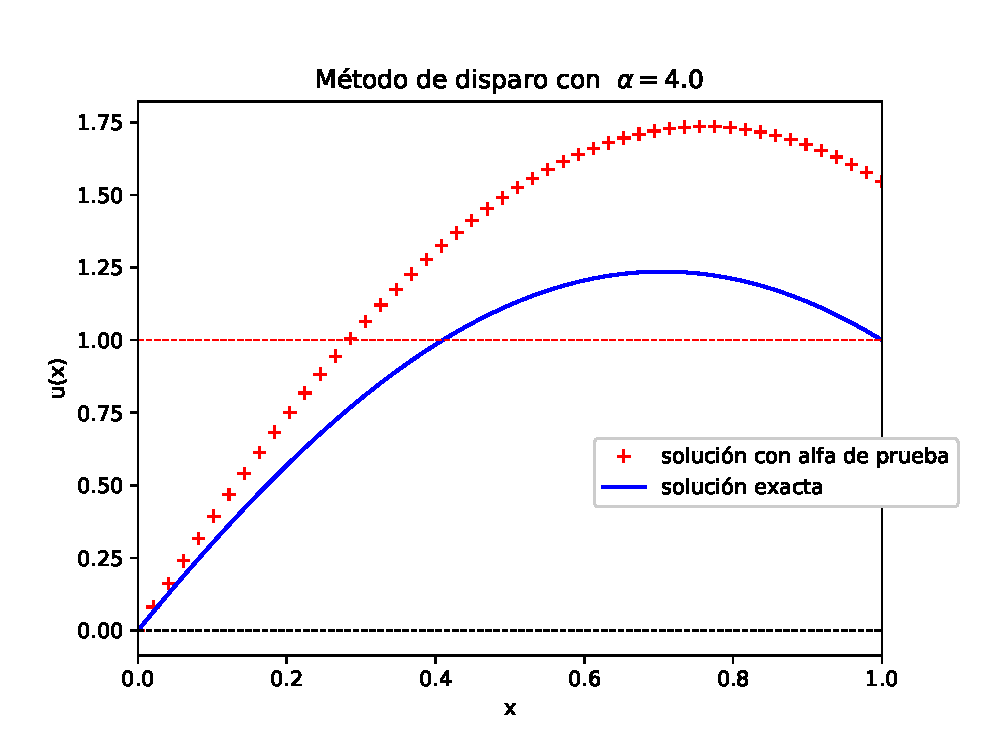
\includegraphics[scale=0.6]{MetodoDisparo2017_02.eps}
\end{figure}
\end{frame}
\begin{frame}
\frametitle{Resultado por arriba}
El cambio del valor de $\alpha = 4.0$ nos devuelve una solución que queda por arriba de lo esperado.
\\
\bigskip
Pensar que si implementamos una rutina que esté incrementado el valor de $\alpha$ de manera automática hasta lograr el valor exacto, es quizá, la manera en la que no debemos de pensar.
\end{frame}
\begin{frame}
\frametitle{¿Qué hacemos?}
El siguiente paso es encontrar el valor de la raíz en donde $f(\alpha) = u_{\alpha}(1) - 1 = 0$.
\\
\medskip
Revisando los valores que obtenemos para $\alpha$:
\\
\medskip
$u_{1.0}(1) = -0.3633$ \\
$u_{4.0}(1) = 1.5464$
\\
\medskip
Por lo que necesariamente hay una raíz que debemos de utilizar para sustituirla en nuestro problema.
\end{frame}
\begin{frame}[fragile]
\frametitle{Interpolando para hallar la raíz}
Dados los valores de la función en dos puntos, podemos utilizar la interpolación con \python, de la siguiente manera:
\begin{lstlisting}[caption=Código para la interpolación, style=FormattedNumber, basicstyle=\linespread{1.1}\ttfamily=\small, columns=fullflexible]
xp = [1.0, 4.0]
fp = [-0.363380, 1.546479]

alfaexacta = np.interp(1.0, , )

print(alfaexacta)
\end{lstlisting}
Revisa cómo deben de ir los argumentos \texttt{xp, fp}, tenemos que aplicar una interpolación inversa.
\end{frame}
\begin{frame}[fragile]
\frametitle{Solución con $y0 = array([0.0,\alpha=3.14159])$}
\begin{figure}
    \centering
    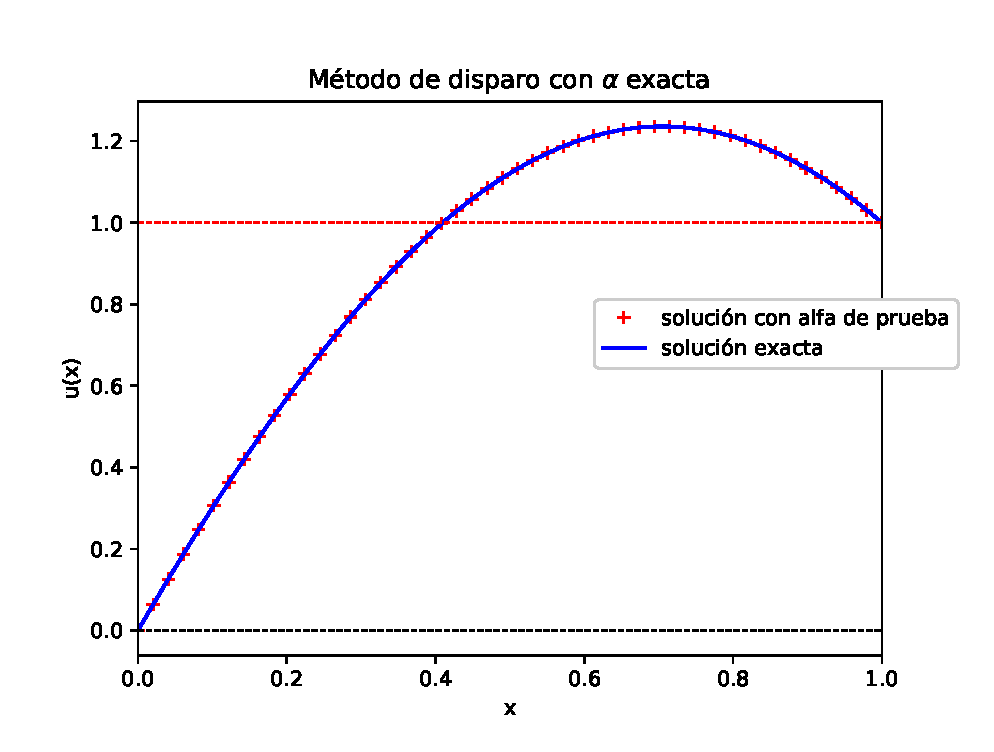
\includegraphics[scale=0.5]{MetodoDisparo2017_03.eps}
\end{figure}
\end{frame}
\end{document}